\documentclass[letterpaper, inpress]{jds} % use this for production
% \documentclass[a4paper, review]{jds}      % use this for review


%%%%%%%%%%%%%%%%%%%%%%%%%%%%%%%%%%%%%%%%%%%%%%%%%%%%%%%%%%%%%%%%%%%%%%
%% the following edits should be done by Journal typesetters
%%%%%%%%%%%%%%%%%%%%%%%%%%%%%%%%%%%%%%%%%%%%%%%%%%%%%%%%%%%%%%%%%%%%%%
\setcounter{page}{1}            % set the first page number
\jdsmonth{July}                 % month
\jdsyear{2020}                  % year
\jdsvolume{xx}                  % volume number
\jdsissue{xx}                   % issue number
\jdsdoi{xx.xxxx/xxxxxxxxx}      % doi
\jdsreceived{April, 2020}       % optional: comment it out if no received date
\jdsaccepted{May, 2020}         % optional: comment it out if no accepted date
%% manually set running header for a shorter list of authors if needed
% \shortauthors{A Author A, et al.}


%%%%%%%%%%%%%%%%%%%%%%%%%%%%%%%%%%%%%%%%%%%%%%%%%%%%%%%%%%%%%%%%%%%%%%
%% edits by authors are given below
%%%%%%%%%%%%%%%%%%%%%%%%%%%%%%%%%%%%%%%%%%%%%%%%%%%%%%%%%%%%%%%%%%%%%%
\usepackage{amsfonts,amsmath,amssymb,amsthm}
\usepackage{booktabs}

\usepackage{lipsum}

\title[Perceptual Judgements on 3D Bar Charts]{Evaluating Perceptual Judgements on 3D Printed Bar Charts}

%% corresponding authors can be labeled by either \thanks or \footnote
\author[1]{Tyler Wiederich\thanks{Corresponding author. Email: twiederich2@huskers.unl.edu}}
\author[1]{Susan VanderPlas\footnote{Corresponding author. Email: susan.vanderplas@unl.edu}}
\affil[1]{Department of Statistics, University of Nebraska-Lincoln}



\begin{document}

\maketitle

\begin{abstract}
  Visual depth is a limiting factor for the interpretation of 3D data visualizations rendered in 2D environments. 
  It is well documented that the accuracy of data comparisons is worse for 3D charts, but these studies are almost entirely focused with 2D projections.
  Our study brings these graphs into a 3D environment and compares the effectiveness of 3D printed charts to their 2D rendered counterparts.
  Primilinary results do not show a difference in judgment accuracy between charts, .\@
\end{abstract}

\begin{keywords} % alphabetical; excluding anything in the title already
  Graphics;
  3D bar charts;
  3D printing
\end{keywords}

\section{Introduction}%
\label{sec:intro}

The goal of our research is to replicate partial results from \cite{cleveland_graphical_1984} and extend their study to multiple mediums of data visualizations.
Current research into 3D data graphics is mostly limited to 2D projections and shows that 3D graphs are less accurate at portraying numeric information than 2D graphs \cite{barfield_effects_1989,fisher_data_1997}.
In certain contexts and conditions, there is some research suggesting that 3D graphs may better encode information \cite{brath_3d_2014}. 

Here, we provide the process of replication and modernization of testing perceptual judgements to 2D graphs, 3D graphs projected in 2D environments, and 3D printed bar graphs.


\subsection{Selected Components From Cleveland and McGill}

Cleveland and McGill provided a theory and tested for the ordering of perceptual importance for the elements of length, position, and angle. 
Their first experiment, referenced as the position-length experiment, used five types of bar charts.
Two of these were grouped bar charts and the other three were stacked bar charts.
Each chart had two bars used for comparison and participants were asked to determine which bar was smaller and give their perceived ratio of the smaller bar to the larger bar.
The two grouped bar charts are for the perceptual element of position along a common scale, where one has zero distance between bars and the other has a fixed distance between bars.
These grouped bar charts will be referenced as adjacent and separated graph types in this paper, respectively.

Our study replicates the procedure for the comparisons of the two grouped bar charts, but with an objective of detecting differences between 2D graphs, 3D digital graphs, and 3D printed graphs.

\section{Methods}

Our study is designed to replicate part of the position-length experiment as closely as possible. 
In this section, we will discuss the replication process and the design of our modified version of the position-length experiment.

\subsection{Replicating Cleveland and McGill}

The first step of replicating the position-length experiment was to determine the values used for comparison. These values for bar heights are linear on a log scale and are given by 
\[s_i=10\cdot 10^{(i-1)/12}, i=1,...,10\]
The ratio of heights between the bars that were compared by Cleveland and McGill were 17.8, 26.1, 38.3, 46.4 (twice), 56.2, 68.1 (twice), and 82.5 (twice). 
The exact numeric comparisons were not disclosed, but the comparison values were subjected to the constraints of having the same ratios and that no value was used more than twice.

Each graph is presented so that there are ten bars. 
Within a graph, only two bars are marked for identification.
Cleveland and McGill did not specifically state the random process for generating the remaining bars of the grouped bar charts, so the remaining bar heights were generated from a scaled Beta distribution with parameters that limit the amount of obsessive noise around the bars used for comparison. The aspect ratio of the plots are approximately 4:3.3, which was determined by measuring the pixels of a figure in Cleveland and McGill's paper. 

\subsection{Designing Graphics}

Due to limitations, creative adjustments were made from Cleveland and McGill's study to closely match both types of 3D charts (digital and 3D printed) to our 2D charts. 
The graphs share a common layout across the three chart types. 
There are two groupings of five bars and each grouping is identified by either "A" or "B". Circles and triangles are used to identify the bars that are to be compared by participants.

\begin{figure}[ht]
  \begin{center}
  \centerline{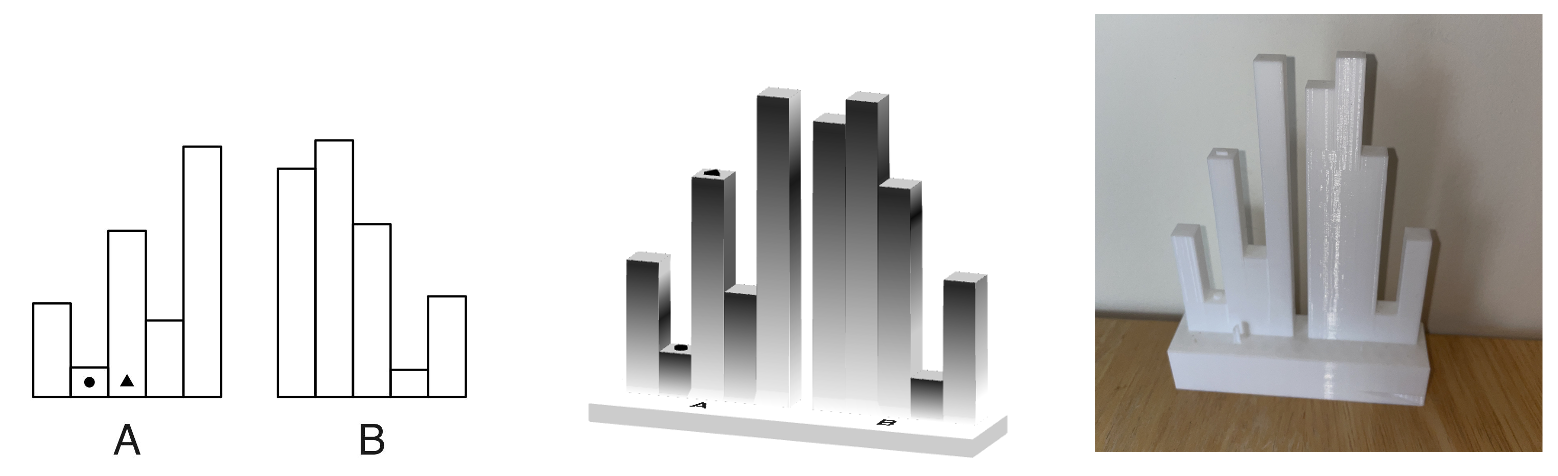
\includegraphics[width=\columnwidth]{chart_types}}
  \caption{A 2D graph, 3D graph, and a prototype 3D printed graph showing the same set of data.}
  \label{chartcomparison}
  \end{center}
  \end{figure}


































\section{Equations}%
\label{sec:eq}


Weibull distribution has the virtue of being a mathematically tractable model
and is versatile in terms of its applications in reliability, life data
analysis, actuarial science and others. Apart from being a potential model in
survival analysis and reliability engineering, it has a vast domain of other
applications.

Equations are always parts of sentences, so they need to have
appropriate punctuations. To evaluate the distribution of a normal
variable, one use
\begin{equation}
  \label{eq:cdf}
  \Pr(Z \le t) = \Phi\left(\frac{Z - \mu}{\sigma} \right),
\end{equation}
where $Z$ follows a $N(\mu, \sigma^2)$ distribution.
Equations can be referenced by \texttt{$\backslash$eqref}.
When $\mu = 0$ and $\sigma = 1$, the $Z$ in Equation~\eqref{eq:cdf}
becomes a standard normal variable.


Multiline equations can be presented with the \texttt{align}
environment. For example,
\begin{align*}
  g_{\mu}(\phi) = 0,\\
  g_{\mu}(X) = 1.
\end{align*}


An equation that is not referenced should not be labeled. The starred
version of the \texttt{equation} and \texttt{align} are for this purpose.

\section{Tables}%
\label{sec:tabs}

We recommend \LaTeX\ package \texttt{booktabs} for professional
looking tables. Its toprule and bottomrule are thicker than midrule.

A professional table contains no vertical lines.

Table~\ref{tab:realdata} is an illustration.
\begin{table}[tbp]
  \caption{Analysis results for real data. Point
    estimates (EST) from both two-piece method and marginal method are
    reported. Standard error of point estimates are evaluated by
    parametric bootstrap (SE).}%
  \label{tab:realdata}
  \centering
  \begin{tabular}{llrrrr}
    \toprule
    \multicolumn{1}{l}{Season} & \multicolumn{1}{l}{Parameter}
    & \multicolumn{2}{c}{Two-piece method} & \multicolumn{2}{c}{Marginal method} \\
    \cmidrule(r){3-4} \cmidrule(r){5-6}
                               & & EST & SE & EST & SE \\
    \midrule
    Summer & $\lambda_1$ & 2.841 & 0.459 & 1.090 & 0.280 \\
   & $\lambda_0$ & 0.179 & 0.014 & 0.158 & 0.015 \\
   & $\sigma$ & 1.335 & 0.106 & 0.999 & 0.104 \\
   & $\sigma_\epsilon (\times 10^{-2})$ & 1.854 & 0.087 & 1.879 & 0.078 \\
  Winter & $\lambda_1$ & 6.225 & 0.825 & 4.720 & 0.711 \\
   & $\lambda_0$ & 0.118 & 0.010 & 0.114 & 0.009 \\
   & $\sigma$ & 1.506 & 0.095 & 1.454 & 0.089 \\
   & $\sigma_\epsilon (\times 10^{-2})$ & 0.908 & 0.036 & 0.934 & 0.043 \\
    \bottomrule
  \end{tabular}
\end{table}




\section{Figures}%
\label{sec:figs}

Vector graphics do not lose clarity when being scaled. Make your
figure in pdf format when you first generate it and keep in mind its
sizes in the article to avoid over-scaling. Do not simply convert a
jpeg or png image to a pdf.

\section{Code}%
\label{sec:code}

The document class \texttt{jds} provides several commands to decorate
\begin{itemize}
\item inline code, such as \code{print("Hello world!")};
\item programming language, such as \proglang{R}, \proglang{Python}, and
  \proglang{C++};
\item software package, such as \pkg{stats}, \pkg{utils}.
\end{itemize}


\section{Guide for Authors}%
\label{sec:guide-authors}

The following requirements must be followed as closely as possible. A
technically acceptable manuscript that fails to follow these requirements may be
returned for retyping, leading to delay in publication.We only accept
submissions in PDF format. The Latex file must be provided after the manuscript
is accepted.

\subsection{Submission of Papers}

Submission of a manuscript must be the original work of the author(s) and have
not been published elsewhere or under consideration for another publication, or
a substantially similar form in any language.

Authors are encouraged to recommend three to five individuals (including their
research fields, e-mail, phone numbers and addresses) who are qualified to serve
as referees for their paper.


% \subsection{Manuscript Preparation}

% All manuscripts should be written in English. Letters are generally no more than
% three journal pages. The supporting organization and the grant number should be
% given at the end of the manuscript. For more details of submission format,
% please visit the website:

% \begin{itemize}
% \item Title: The title of the paper should be concise but informative.
% \item Author name(s): A list of all authors, as well as corresponding addresses,
%   should be provided on the title page. Authors’ names should be given in a
%   consistent form on all publications to facilitate indexing. It will be better
%   if the fax number(s), e-mail address(es), and telephone number(s) are all
%   provided.
% \item Abstract: The abstract should be no longer than 100 words. It should be
%   informative, without descriptive words or citations, and contain the major
%   conclusions and quantitative results or other significant items in the
%   paper. Together with the title, the abstract must be adequate as an index to
%   all the subjects treated in the paper, and will be used as a base for
%   indexing.
% \item Main body of the paper: The body of the paper should include all the
%   information of the research, but no subtitles.
% \item Formulas: Formulas should be punctuated and aligned to bring out their
%   structure, and numbered consecutively in round brackets on the right-hand side
%   of the page.
% \item Notation: Notation must be legible, clear, compact, and consistent with
%   standard usage. All unusual symbols whose identity may not be obvious,
%   including subscript or superscript, must be made comprehensible. Physical and
%   mathematical variables should be in italic, vectors in boldface. Units,
%   abbreviations and special functions should be upright. Please add notes to
%   explain any other special symbols.
% \item Figures: Figures should be original laser prints with high contrast,
%   suitable for immediate reproduction, typed on separate sheets and identified
%   by its number. They will normally be reduced to one column width (6--8 cm). In
%   the figures, the main lines should be about 0.3 mm in width, and the assistant
%   lines 0.15 mm. Notations in the figures should be distinct and consistent with
%   the same ones in the text, and their font size will be 7--9 pt. The positions
%   of figures should be marked in the text by boxes of a suitable size. Each
%   figure should have its own caption. For photographs, the original photos must
%   be supplied with good contrast and clearly distinguishable details.
% \item Tables: Tables, numbered in order of appearance, should be appended on
%   separate sheets and identified with appropriate titles.The table title, which
%   should be brief, goes above the table. A detailed description of its contents
%   or table footnotes should be given directly below the body of the table.
% \item References: References must be published work, and numbered consecutively
%   in order of their first citation. References should be listed individually at
%   the end of the text and indicated in the text with a superscript number in
%   square brackets. All of the references’ authors, as well as the titles of the
%   referenced articles, should be given.
% \item Proofs: Authors will receive a letter informing them whether the
%   manuscript is accepted or rejected in two months. Authors should return their
%   revisions to the Manuscript Office within one month on receipt. When an
%   article has been amended in compliance with the comments of referee(s), an
%   electronic file of the final version should be sent with the revised
%   manuscript. Proofs will be sent to the authors and should be returned
%   preferably within 48 hours to avoid publication delays.
% \end{itemize}


\section{A Placeholder Section}%
\label{sec:placeholder}

\lipsum[4-7]

\section{Citing References}%
\label{sec:citations}

The citations are in the author-year format with the
\texttt{chicago} bibstyle.

A bibfile contains all the citations in
bibtex format is prepared (see \texttt{JDSbib.bib}). Some characters
in the title of the references needs to be protected so that the style
file does not alter it. For example, in the bibtex entry for
\citet{Pozd:etal:2017}, the ``B'' in ``Brownian'' and the ``E'' in
``estimation''  following the colon are protected.
A book reference \citep[e.g.,][]{Kotz2001} should have an address field.


Citations can be in either text or parenthesis format style with
\texttt{$\backslash$citet} or \texttt{$\backslash$citep},
respectively. For example, \citet{KoenkerBassett1978} is a seminal
work on quantile regression; The Laplace distribution has applications
in many fields \citep{Kotz2001}.


\section{Discussion}

\lipsum[1-3]

\bibliographystyle{jds}
\bibliography{JDS2023}


\end{document}
